% 	Name		:: 	sthlm Beamer Theme  HEAVILY based on the hsrmbeamer theme (Benjamin Weiss)
%	Author		:: 	Mark Hendry Olson (mark@hendryolson.com)
%	Created		::	2013-07-31
%	Updated		::	June 18, 2015 at 08:45
%	Version		:: 	1.0.2
%	Email		:: 	hendryolson@gmail.com
%	Website		:: 	http://v42.com
%
% 	License		:: 	This file may be distributed and/or modified under the
%                  	GNU Public License.
%
%	Description	::	This presentation is a demonstration of the sthlm beamer
%					theme, which is HEAVILY based on the HSRM beamer theme created by Benjamin Weiss
%					(benjamin.weiss@student.hs-rm.de), which can be found on GitHub
%					<https://github.com/hsrmbeamertheme/hsrmbeamertheme>.


%-=-=-=-=-=-=-=-=-=-=-=-=-=-=-=-=-=-=-=-=-=-=-=-=
%
%        LOADING DOCUMENT
%
%-=-=-=-=-=-=-=-=-=-=-=-=-=-=-=-=-=-=-=-=-=-=-=-=

\documentclass[newPxFont]{beamer}
\usetheme{sthlm}
%\usecolortheme{sthlmv42}

%-=-=-=-=-=-=-=-=-=-=-=-=-=-=-=-=-=-=-=-=-=-=-=-=
%        LOADING PACKAGES
%-=-=-=-=-=-=-=-=-=-=-=-=-=-=-=-=-=-=-=-=-=-=-=-=
\usepackage[utf8]{inputenc}
\usepackage[T1]{fontenc}

%\usepackage{chronology}
\usepackage{chronosys}
\usepackage{subfigure}

\newcommand{\tabitem}{%
  \usebeamertemplate{itemize item}\hspace*{\labelsep}}

%\renewcommand{\event}[3][e]{%
%  \pgfmathsetlength\xstop{(#2-\theyearstart)*\unit}%
%  \ifx #1e%
%    \draw[fill=black,draw=none,opacity=0.5]%
%      (\xstop, 0) circle (.2\unit)%
%      node[opacity=1,rotate=45,right=.2\unit] {#3};%
%  \else%
%    \pgfmathsetlength\xstart{(#1-\theyearstart)*\unit}%
%    \draw[fill=black,draw=none,opacity=0.5,rounded corners=.1\unit]%
%      (\xstart,-.1\unit) rectangle%
%      node[opacity=1,rotate=45,right=.2\unit] {#3} (\xstop,.1\unit);%
%  \fi}%

%-=-=-=-=-=-=-=-=-=-=-=-=-=-=-=-=-=-=-=-=-=-=-=-=
%        BEAMER OPTIONS
%-=-=-=-=-=-=-=-=-=-=-=-=-=-=-=-=-=-=-=-=-=-=-=-=

%\setbeameroption{show notes}

%-=-=-=-=-=-=-=-=-=-=-=-=-=-=-=-=-=-=-=-=-=-=-=-=
%
%	PRESENTATION INFORMATION
%
%-=-=-=-=-=-=-=-=-=-=-=-=-=-=-=-=-=-=-=-=-=-=-=-=

\title{Repenser la gouvernance des systemes complexes : la question de la place des humains dans leurs milieux}
%\subtitle{A sensitive common threatened by uncertainty in intensification process}
%\date{\small{\jobname}}
%\date{\today}
\date{Novembre 2019}
\author{\texttt{E. Delay, J.-P. Müller, S. Aubert \\ Discutantes : M.-H. Durand}}
\institute{CIRAD -- UPR GREEN}

\hypersetup{
pdfauthor = {E. DELAY},
pdfsubject = {Chantier Communs 2},
pdfkeywords = {Séminaire de restitution au Pôle foncier (Montpellier)},
pdfmoddate= {D:\pdfdate},
pdfcreator = {}
}

\begin{document}

%-=-=-=-=-=-=-=-=-=-=-=-=-=-=-=-=-=-=-=-=-=-=-=-=
%
%	TITLE PAGE
%
%-=-=-=-=-=-=-=-=-=-=-=-=-=-=-=-=-=-=-=-=-=-=-=-=


\maketitle

%\begin{frame}[plain]
%	\titlepage
%\end{frame}

%-=-=-=-=-=-=-=-=-=-=-=-=-=-=-=-=-=-=-=-=-=-=-=-=
%
%	TABLE OF CONTENTS: OVERVIEW
%
%-=-=-=-=-=-=-=-=-=-=-=-=-=-=-=-=-=-=-=-=-=-=-=-=
% \section*{Une bousole ?}
% \begin{frame}{Overview}
% % For longer presentations use hideallsubsections option
% \tableofcontents[hideallsubsections]
% \end{frame}

%-=-=-=-=-=-=-=-=-=-=-=-=-=-=-=-=-=-=-=-=-=-=-=-=
%	FRAME: INTRODUCTION
%-=-=-=-=-=-=-=-=-=-=-=-=-=-=-=-=-=-=-=-=-=-=-=-=

\section{Introduction : modeliser dans l'urgence}


\begin{frame}[c]{L'urgence socio-environnementale}
\vspace{-1cm}
À l'échelle mondiale, de nombreux facteurs peuvent empêcher les populations d'avoir accès aux ressources fondamentales de leur existence :
\begin{itemize}
  \item faits de violence et de guerre,
  \item appropriation des terres au Sud,
  \item artificialisation au Nord,
  \item \textit{etc.}
\end{itemize}
\begin{figure}
  \includegraphics[height=3cm]{img/Honduras.jpg}
  \caption{\textit{Dépaysage au Honduras}, Agnès Stienne, 2019}
\end{figure}
\end{frame}

\begin{frame}[c]{Doomed ?}
\vspace{-1cm}

\begin{figure}
  \includegraphics[width=\textwidth]{img/im_legend-600.jpg}
  \caption{I'm a legend (film, 2007)}
\end{figure}
\end{frame}

\begin{frame}[c]{Un sentier, une piste, une autoroute ... ?}
\vspace{-1cm}
\begin{figure}
  \includegraphics[height=3.5cm]{img/cyrano.jpg}
  \caption{Cyrano de Bergerac (film 1990)}
\end{figure}
\begin{itemize}
  \item Depuis Ostrom (1990), une forte dynamique autour des Communs,
  \item Une dynamique qui réinterroge la condition de l’homme dans le système.
\end{itemize}
\end{frame}

\begin{frame}[c]{Modéliser les Communs de la terre}
\vspace{-1cm}
La démarche de modélisation de l’approche peut être formalisée en 4 étapes :

\begin{itemize}
  \item la notion même de système permet de mieux caractériser les situations d’action
  \item la notion de complexité pour définir les communs en considérant les concepts d’émergence faible et forte,
  \item la modélisation des systèmes complexes constitue un moyen de conscientisation,
  \item la production normative dans ce contexte résulte essentiellement de l’usage; la gouvernance des systèmes complexes passe par la conceptualisation
\end{itemize}

\end{frame}

\begin{frame}[c]{Mais pourquoi modéliser ?}
\vspace{-1cm}

Qu'est-ce qu'un modèle ?
\begin{itemize}
  \item `` A* est un modèle de A si manipuler A* permet de répondre à la question (ou l'objectif) Q sur A posée par X '' (Minsky 1965)
\end{itemize}

Pourquoi faire ?
\vspace{-0.4cm}
\begin{figure}
  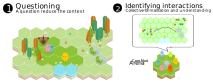
\includegraphics[height=3.2cm]{img/modeliser.png}
\end{figure}

\small{
  \begin{alertblock}{\textsc{Une hypothese forte}}
    La déconstruction de la réalité sous la forme abstraite de modèle va permettre aux différents acteurs concernés de mieux saisir et expliciter les relations entre les composants du système.
  \end{alertblock}
}
% \begin{figure}
%   \includegraphics[height=3.5cm]{img/pict_cyril_piou.jpg}~\includegraphics[height=3.5cm]{img/pict_etienne_delay.jpg}
% \end{figure}
\end{frame}

%-=-=-=-=-=-=-=-=-=-=-=-=-=-=-=-=-=-=-=-=-=-=-=-=
%	FRAME: LA NOTION DE SYSTÈME ET DE SYSTÈMES COMPLEXES
%-=-=-=-=-=-=-=-=-=-=-=-=-=-=-=-=-=-=-=-=-=-=-=-=

\section{La notion de systeme complexe}

\begin{frame}[c]{Le système et ses limites}
\vspace{-1cm}
Un système = (au moins) un observateur qui délimite
\begin{itemize}
  \item Posture réaliste : le système pré-existe à l'observateur et s'impose (Pseudo-communs (Theesfled, 2019))
  \item Posture épistémique : c'est l'observateur, la situation d'action, qui va délimiter le système (relation, interactions) (Ostrom, 1990; Haller, 2019).
\end{itemize}

\small{
  \begin{alertblock}{\textsc{Positionnement epistemique}}
      Le commun n'est pas, il devient.
  \end{alertblock}
}

En explicitant le système; son dedans et son dehors $\rightarrow$  conscientisation les limites est une condition nécessaire à sa définition.

% \begin{figure}
%   \includegraphics[height=3.5cm]{img/stienne2018_square.jpg}
%   \caption{A. Steinne, 2018, Plantaciones y pradera florida.}
% \end{figure}

\end{frame}

\begin{frame}[c]{Le système et les interactions}
\vspace{-1cm}
Un système c'est :
\begin{itemize}
  \item des composantes (humain et non humain)
  \item des relations entre ses composantes
\end{itemize}

\small{
  \begin{alertblock}{\textsc{Le triptyque}}
      Entrer par les relations structure des triptyques usagés $\rightarrow$ usage $\rightarrow$ ressource. La frontière du système se reconfigure au gré des interactions/relations.
  \end{alertblock}
}
\begin{figure}
  \includegraphics[height=3.5cm]{img/ReHab_network.png}
\end{figure}

\end{frame}


\begin{frame}[c]{La complexité}
\vspace{-1cm}
\begin{itemize}
  \item Un système est complexe lorsque les interactions entre les composants sont non linéaires (J.-P. Müller, 2004), c'est à dire,  lorsque les effets ne peuvent s’additionner.
  \item Les interactions non linéaires ont la propriété de faire émerger un comportement au niveau du système considéré.
\end{itemize}


\begin{figure}
  \includegraphics[height=3.5cm]{img/anatomical-illustration-of-the-human-brain.jpg}
\end{figure}
\end{frame}

% \begin{frame}[c]{L'emergence et les Communs de la terre}
% \vspace{-1cm}
% Il y a émergence si et seulement si :
% \begin{itemize}
%   \item Un observateur a identifié un système (et sa frontière), donc ses composants et leursinteractions sous la forme d’une théorie D (par exemple, l'exercice des usages de la terre et des ressources naturelles dans un même milieu - les pratiques des usagers) ;
%   \item La production d’un comportement global au niveau du système (par exemple, la récurrence des comportements collectifs d’accès à la terre et aux ressources ) ;
%   \item L’observation de ce comportement global par un observateur (qui peut être le même) et sa description dans une théorie D’ (par exemple, les règles de distribution des ressources qui décrivent ces réccurrences) ;
%   \item L’irréductibilité de la théorie D’ à la théorie D (Bunge 1977).
% \end{itemize}
% \end{frame}

\begin{frame}[c]{Deux types d'emergence}
\vspace{-1cm}
On peut distinguer l’émergence faible de l’émergence forte

\begin{figure}
  \includegraphics[height=3.5cm]{img/Screenshot_2019-11-18 (143) Lucy's Famous Chocolate Scene - YouTube}
  \caption{Lucy's Famous Chocolate Scene (1950)}
\end{figure}

\small{
  \begin{alertblock}{\textsc{Auto-organisation}}
      L'émergence forte permet de maintenir les caractéristiques globales du système et donc les composants, leurs interactions et la frontière à l’origine de cette émergence. On parle alors d’auto-organisation et le système devient homéostatique.
  \end{alertblock}
}

\end{frame}


% \begin{frame}[c]{Les outils des systèmes complexes}
% \vspace{-1cm}
% %
% % les systèmes complexes sont construits sur une analyse à deux niveaux :
% % \begin{itemize}
% %   \item le niveau macroscopique du comportement global du système. Qui peuvent représenter \textbf{les collectifs d’usagers}. Hypothèse d'atomicité.
% %   \item le niveau microscopique des composants en interaction (et possiblement avec un extérieur donc une frontière explicite), qui peuvent être les \textbf{usagers}. S'abstrait de l'hypothèse d'atomicité,
% % \end{itemize}
%
% % Les Systèmes Multi-Agents (SMA) qui, quoique moins formellement caractérisés que les équations, représentent de mainère plus descriptive les composantes du système.
%
% Un système multi-agent
% \begin{itemize}
%   \item est un ensemble d’agents (entités physiques ou virtuelles)
%   \item en interactions entre eux (structure en réseau)
%   \item possiblement dans et avec un environnement (agents spatialement situés),
%   \item muni d’un comportement qui consiste à engendrer des forces ou des actions vers les autres agents et possiblement l’environnement sur la base des forces ou des perceptions.
% \end{itemize}
%
% \end{frame}
%-=-=-=-=-=-=-=-=-=-=-=-=-=-=-=-=-=-=-=-=-=-=-=-=
%	FRAME: MODÉLISER LES SYSTÈMES COMPLEXES
%-=-=-=-=-=-=-=-=-=-=-=-=-=-=-=-=-=-=-=-=-=-=-=-=

%\section{Modeliser\\les systemes complexes}


%-=-=-=-=-=-=-=-=-=-=-=-=-=-=-=-=-=-=-=-=-=-=-=-=
%	FRAME: GOUVERNER LES SYSTÈMES COMPLEXES
%-=-=-=-=-=-=-=-=-=-=-=-=-=-=-=-=-=-=-=-=-=-=-=-=

\section{Gouverner les systemes complexes}

% \begin{frame}[c]{Saisir le$\cdot$s commun$\cdot$s}
% \vspace{-1cm}
%
% \small{
%   \begin{block}{\textsc{leitmotiv}}
%       Il existe autant de Communs que de collectifs d’usagers des ressources, et le Commun n’existe pas, mais le devient, par l’usage et les règles toujours ré-actualisées qui permettent de le réguler.
%   \end{block}
% }
%
% Pour les saisir il faut donc monter en abstraction pour décrire les dynamiques de co-gestion/gouvernance qui conduisent à “coordonner” les usages des ressources territorialisées $\rightarrow$ auto-reproduction.
%
% \end{frame}

\begin{frame}[c]{Observation, perception intérieure/extérieure}
\vspace{-1cm}

\begin{figure}
  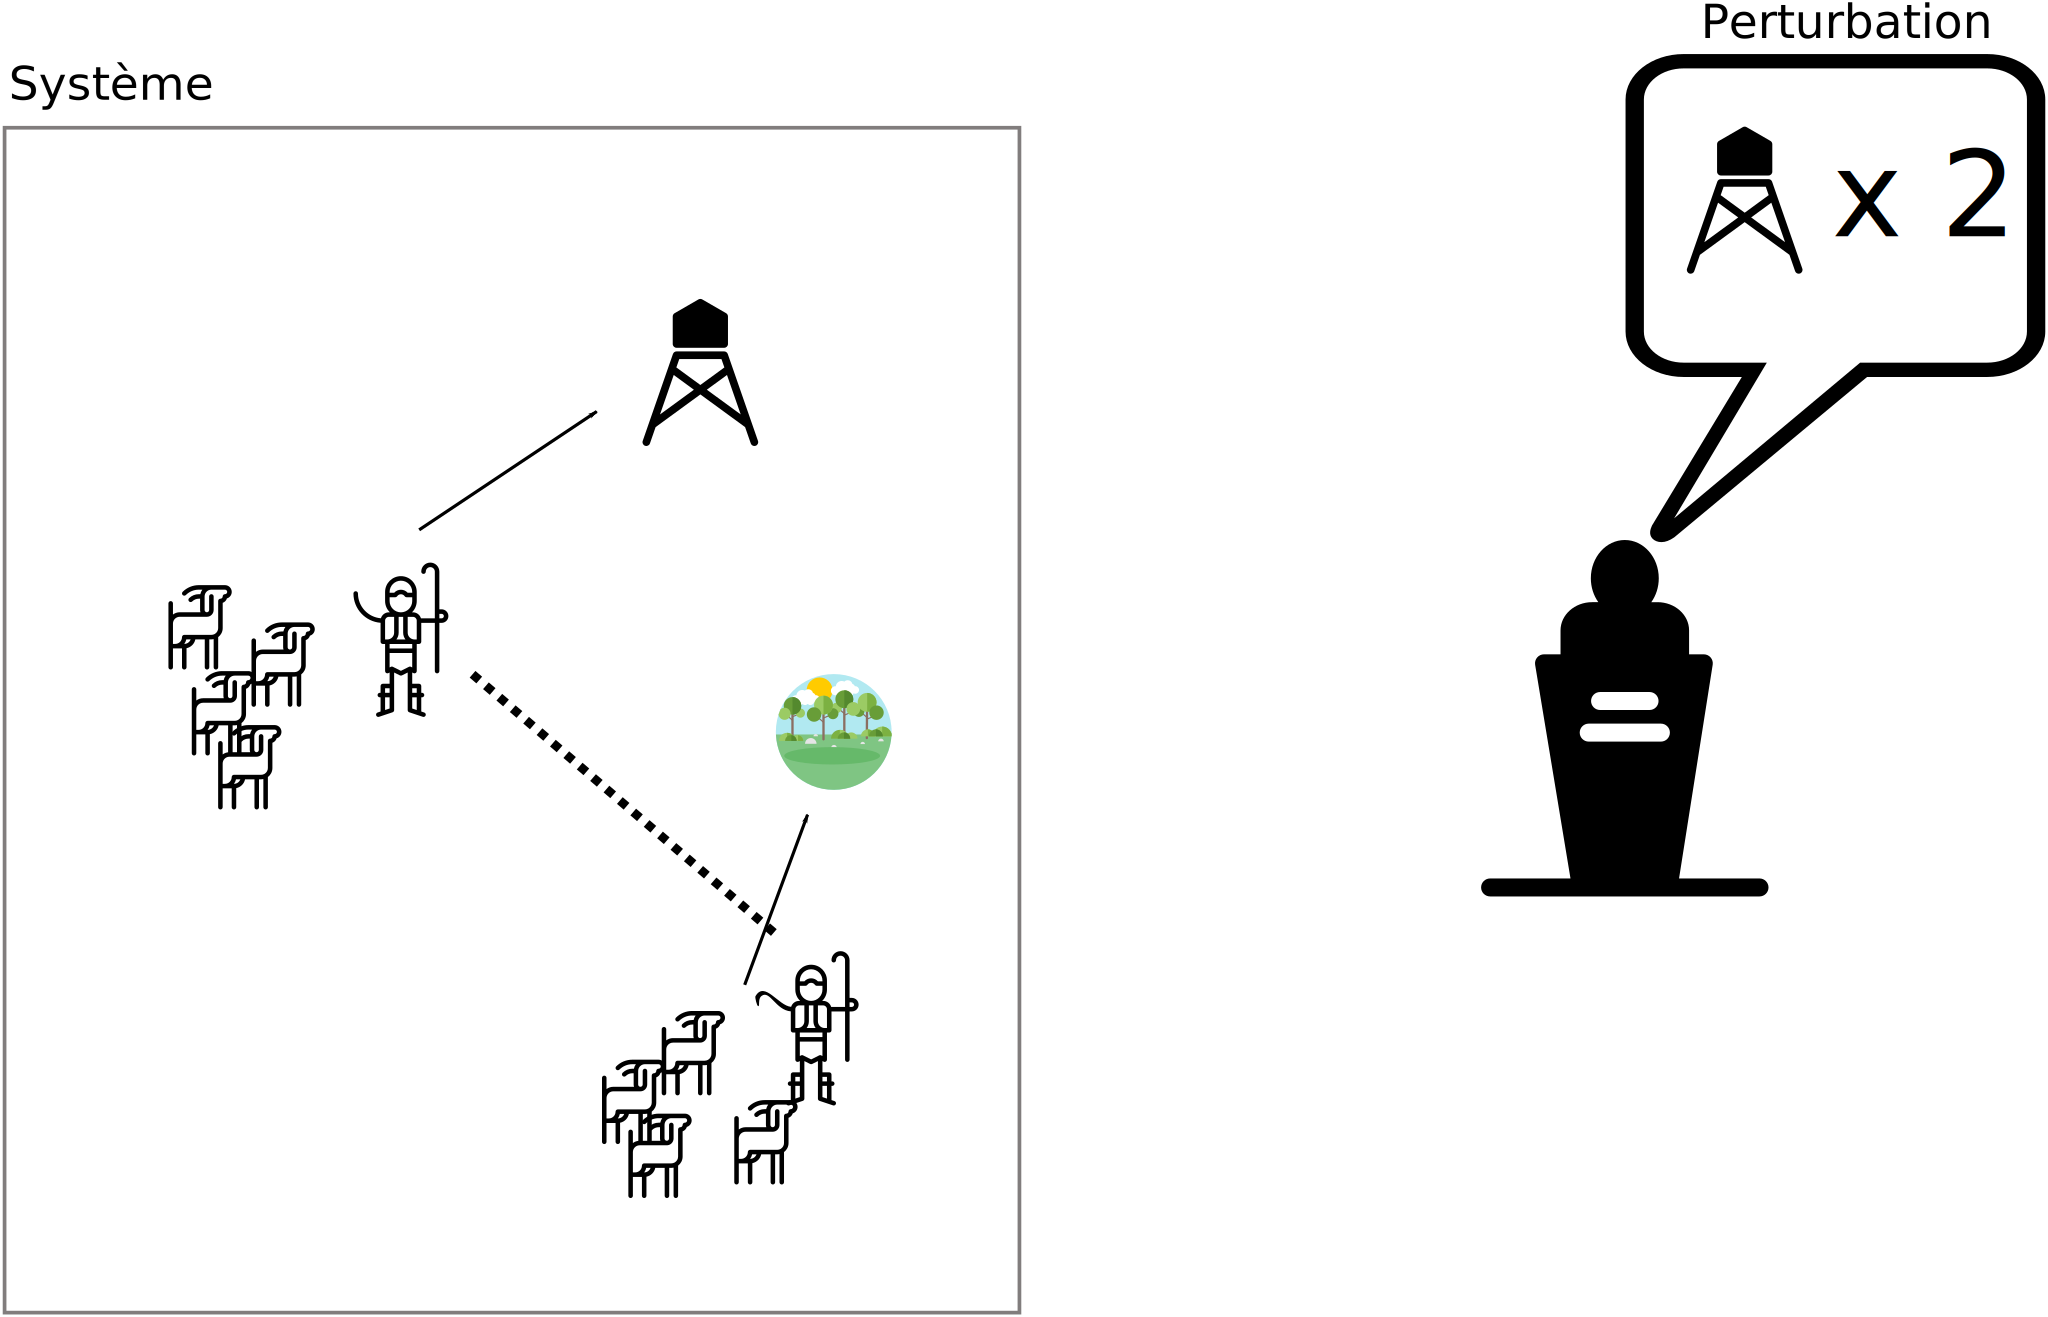
\includegraphics[height=4cm]{img/Systeme_perception.png}
\end{figure}
\begin{itemize}
  \item Les interactions peuvent être le support de chaînes causales de l’intérieur vers l’extérieur du système.
  \item Les interactions peuvent être le support de chaînes causales de l’extérieur vers l’intérieur du système.
\end{itemize}

C'est quand les interactions sont le support de chaînes causales de l’extérieur vers l’intérieur, que le système perçoit son milieu.

\end{frame}

\begin{frame}[c]{Les effets de l'auto-reproduction}
\vspace{-1cm}

 l’auto-reproduction porte en elle le germe de sa propre contradiction
 \begin{itemize}
   \item la formalisation des organisations informelles $\rightarrow$ réduire ses capacités d'adaptation à des changements rapides (Chevallier, 2011),
   \item Le degré de fermeture ou de clôture du système est un signe de maturité (Auriac, 2000)
 \end{itemize}


 \small{
   \begin{alertblock}{\textsc{Une hypothese forte}}
     il s’agira donc pour les composants du système de produire des règles et des formalismes qui permettent une organisation fluide au sein des groupes d’utilisateurs, sans pour autant les condamner à la sénilité par des structures trop contraintes
   \end{alertblock}
 }

\end{frame}

\begin{frame}[c]{Gouverner les systèmes complexes}
\vspace{-1cm}

\begin{figure}
  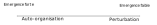
\includegraphics[width=\textwidth]{img/gradiant_emergence.png}
\end{figure}
\vspace{-1cm}
\begin{table}
  \begin{tabular}{c|c}
    Auto-organisation, \textit{etc.}. & perturbation
  \end{tabular}
\end{table}

\begin{figure}
  \includegraphics[width=0.7\textwidth]{img/gouverner.png}
\end{figure}

 \small{
   \begin{alertblock}{\textsc{Perturber le systeme}}
     Pour gouverner depuis l'extérieur $\rightarrow$ envoyez des perturbations qui font sens pour les composantes
   \end{alertblock}
 }
\end{frame}

\begin{frame}[c]{Des formes de gouvernance}
\vspace{-1cm}
Exemples d'effets de perturbation sur la gouvernance des communs :
\begin{itemize}
  \item  réinterprétation des règles produites par les collectifs
  \item  renvoie en retour d’informations utiles pour permettre aux composants d’envisager une nouvelle adaptation de son comportement,
  \item d'autres formes de perturbation à découvrir/inventer
\end{itemize}

 \small{
   \begin{alertblock}{\textsc{Qu'est-ce qui propulse le systeme : les valeurs }}
    Cet éthos (Weber et Bailly (1991)) devient le moteur social/sociétal qui, s’il disparaît, vide le modèle de production de normes de sa légitimité. Si le système a été envisagé avec des composants “législateurs” externes au système, le contrat de confiance entre eux et les acteurs/composants du système implique un consentement préalable (ou des mesures de coercition).
   \end{alertblock}
 }
\end{frame}

\begin{frame}[c]{Attention aux rapports de forces}
\vspace{-1cm}
Les rapports de force sont facilités quand le système ignore certaines parties de lui-même (absence d'émergence forte).

$\rightarrow$  Si l'émergence forte est possible, des comportements malvenus peuvent être saisis par l’ensemble des composants et ceux-ci peuvent mobiliser les solidarités sociales et écologiques pour les entraver (les réguler). Là encore ces solidarités sont basées sur l’éthos et les valeurs du collectif.

\begin{figure}
  \includegraphics[height=4cm]{img/valeurs.jpg}
\end{figure}


\end{frame}

%-=-=-=-=-=-=-=-=-=-=-=-=-=-=-=-=-=-=-=-=-=-=-=-=
%	FRAME: MERCI DE VOTRE ATTENTION
%-=-=-=-=-=-=-=-=-=-=-=-=-=-=-=-=-=-=-=-=-=-=-=-=
{
\usebackgroundtemplate{
\includegraphics[width=\paperwidth]{img/fin}}%
\begin{frame}
  \vspace{-1em}
  \begin{minipage}[t][.8\textheight]{\textwidth}
    \color{\cnGrey}{\LARGE{Merci de votre attention}}

    \vfill

  %\hfill \small{Photo credit : Thomas m-louis. sur \includegraphics[height=0.55cm]{img/flickr_logo}}
  \end{minipage}
  \vspace{-3.5em}
  \centering
	You can find this presentation on github\includegraphics[height=0.85cm]{img/github}

\end{frame}
}


\end{document}
